\documentclass{beamer}
\usetheme{Boadilla}

% to get the handout
% \documentclass[handout]{beamer}
% \usepackage{pgfpages}
% \pgfpagesuselayout{4 on 1}[a4paper,landscape, border shrink=5mm]
% \pgfpageslogicalpageoptions{1}{border code=\pgfusepath{stroke}}
% \pgfpageslogicalpageoptions{2}{border code=\pgfusepath{stroke}}
% \pgfpageslogicalpageoptions{3}{border code=\pgfusepath{stroke}}
% \pgfpageslogicalpageoptions{4}{border code=\pgfusepath{stroke}}
% \usetheme{default}

\usepackage[utf8]{inputenc}
\usepackage{fontawesome}
\usepackage{natbib}
\usepackage{amsfonts}	% for matrices
\usepackage{amsmath}
\usepackage{lipsum}	% used for the unnumbered footnotes
\usepackage[makeroom]{cancel}
\usepackage{tabularx}
\usepackage{pythonhighlight}


\usecolortheme{seagull}

% \AtBeginSection[]
% {
%   \begin{frame}
%     \frametitle{Table of Contents}
%     \tableofcontents[currentsection]
%   \end{frame}
% }

\newcommand{\btVFill}{\vskip0pt plus 1filll}

\newcommand{\light}[1]{\textcolor{gray}{#1}}
\newcommand{\red}[1]{\textcolor{red}{#1}}

\newcommand\blfootnote[1]{%
  \begingroup
  \renewcommand\thefootnote{}\footnote{#1}%
  \addtocounter{footnote}{-1}%
  \endgroup
}

\DeclareMathOperator*{\argmax}{arg\,max}

%Information to be included in the title page:
\title{DIT gentle introduction to Python}
\subtitle{v 2.2 (PhD) January 2023}
\author{Alberto Barr\'on-Cede\~no}
\institute[DIT--UniBO]{Alma Mater Studiorum-Universit\`a di Bologna \\
\texttt{a.barron@unibo.it\hspace{10mm}@\_albarron\_}
}

\date{16/01/2023}

% logo of my university
\titlegraphic{%
\includegraphics[width=2cm]{img/unibo_forli.png}\hspace*{4.75cm}
%
\centering
   
\includegraphics[width=15mm]{img/unibo_forli.png}
}

\begin{document}

\frame{\titlepage}

\begin{frame}
\frametitle{Table of Contents}
\tableofcontents
\end{frame}


\begin{frame}
\section{Basics}
\centering
\alert{Basics}
\end{frame}


\begin{frame}
\frametitle{What is a programming language?}


A programming language is \red{just another language}\ldots
\medskip 					\pause 

\begin{quote}
A formal language comprising a set of \red{instructions} that produce various 
kinds of \red{output} [given an input]
\end{quote}
\begin{flushright}
\footnotesize
 \light{\url{https://en.wikipedia.org/wiki/Programming_language}}
\end{flushright}			\pause 

\bigskip 
\begin{center}
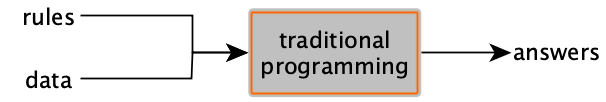
\includegraphics[width=100mm]{img/coli2020_diagrams_traditional_programming.png}
\end{center}

\btVFill
\footnotesize
\light{Diagram borrowed from L. Moroney's Introduction to TensorFlow for 
Artificial Intelligence, Machine Learning, and Deep Learning}

\end{frame}

\begin{frame}
\frametitle{What is a programming language?}

\begin{quote}
Programming languages are used in computer programming to implement an 
\red{algorithm}$^*$
\end{quote}
\begin{flushright}
\footnotesize
 \light{\url{https://en.wikipedia.org/wiki/Programming_language}}
\end{flushright}
\pause 

\begin{columns}
\begin{column}{0.4\textwidth}
\begin{center}
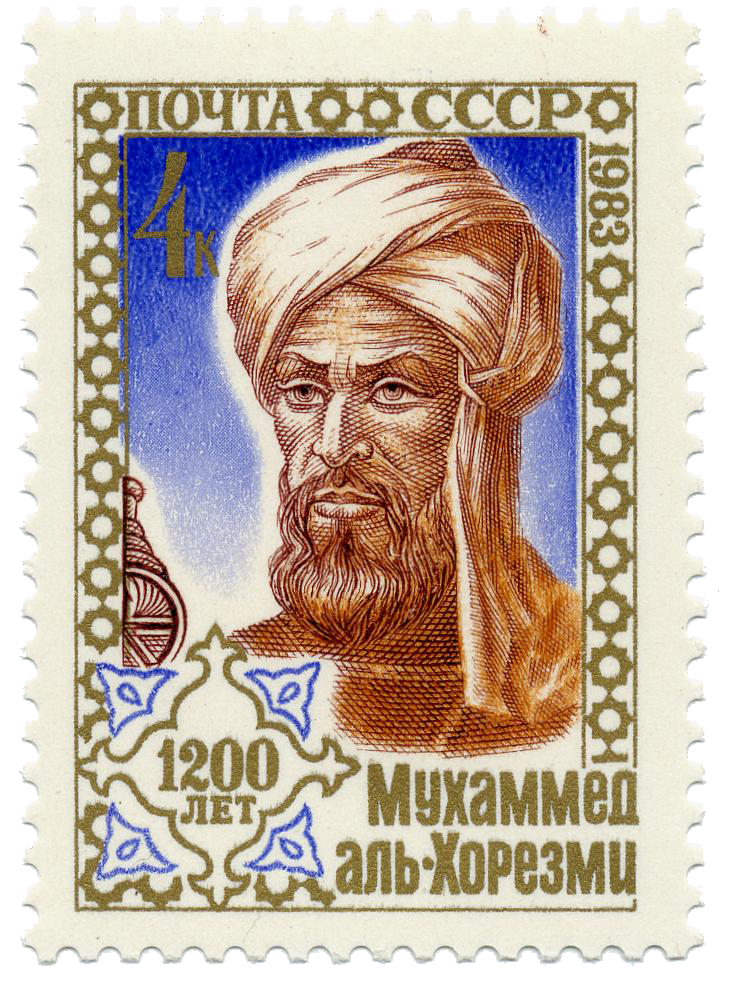
\includegraphics[width=23mm]{img/1983_CPA_5426.png}
\end{center}
\footnotesize
\light{1983 USSR stamp commemorating al-Khwārizmī's (approximate) 1200th 
birthday}
\end{column}

\begin{column}{0.55\textwidth}

$^*$ derived from the 9th century Persian Mathematician Muhammad ibn Mūsā 
al-Khwārizmī
\vspace{10mm}
\end{column}
\end{columns}
\end{frame}

\begin{frame}
\frametitle{The \textit{first} programmer}

\begin{columns}
\begin{column}{0.4\textwidth}
\begin{center}
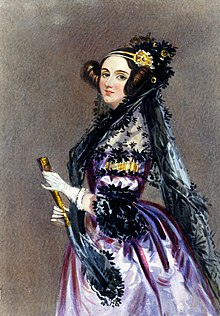
\includegraphics[width=43mm]{img/Ada_Lovelace_portrait.jpg}

\footnotesize
\light{A. Lovelace by 1840}
\end{center}
\end{column}

\begin{column}{0.55\textwidth}

\alert{Ada Lovelace}%
\footnote{Lord Byron’s daughter}
(Mathematician) published the first algorithm for Charles 
Babbage’s \red{analytical engine}

\begin{center}
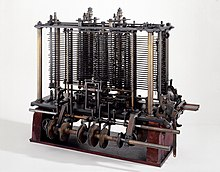
\includegraphics[width=43mm]{img/Babbages_Analytical_Engine_1834-1871.jpg}
\end{center}

\end{column}
\end{columns}
\end{frame}


\begin{frame}
\section{Algorithms}
\centering
\alert{Algorithms}
\end{frame}

\begin{frame}
\frametitle{Algorithm}

\begin{quote}
 A finite sequence of \red{well-defined computer-implementable} instructions, 
typically to solve a class of problems or to perform a computation
\end{quote}
\begin{flushright}
\footnotesize
 \light{\url{https://en.wikipedia.org/wiki/Algorithm}}
\end{flushright}
\end{frame}

\begin{frame}
\frametitle{Algorithm Example: Find out if a number is odd or 
even$^*$}
\pause 

\alert{Definitions}

\begin{itemize}
 \item A number is \red{even} if it can be divided by 2 without remainder
 \item A number is \red{odd} if it leaves a remainder when divided by 2
\end{itemize}				\pause 

\alert{Examples}

\begin{description}
 \item[Even numbers:] 2, 4, 6, 8, etc. 
 \item[Odd numbers:] 1, 3, 5, 7, etc.
\end{description}			\pause 

\alert{Silly (useless) solution:}

\begin{itemize}
 \item Fill a bag with all even numbers and a second bag with all odd numbers
 \item Given an input number, look for it in both bags and return the label of 
the one in which you found it
\end{itemize}	

\btVFill
\onslide
\footnotesize
\light{$^*$Adapted from 
\url{https://www.c-programming-simple-steps.com/algorithm-examples.html}}
\end{frame}

\begin{frame}
\frametitle{Algorithm Example: Find out if a number is odd or even}
\framesubtitle{Problem Definition}
\begin{columns}

\begin{column}{0.5\textwidth}
\red{Input/Output}

$\rightarrow$ an integer\,\,\,\,(data)

$\leftarrow$ even or odd 	(more data)	\pause 

\bigskip
\red{Process}

A series of instructions and routines
\end{column}

\begin{column}{0.4\textwidth}
\begin{center}
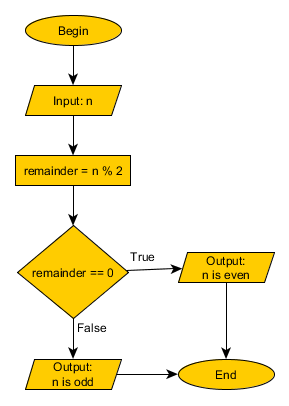
\includegraphics[width=43mm]{img/even-or-odd.png}
\end{center}
\end{column}
\end{columns}
\btVFill
\onslide
\footnotesize
\light{Diagram borrowed from 
\url{https://www.c-programming-simple-steps.com/algorithm-examples.html}}
\end{frame}


\begin{frame}[fragile]
\frametitle{Algorithm Example: Find out if a number is odd or even}
\framesubtitle{From the algorithm to the implementation }

\begin{columns}

\begin{column}{0.5\textwidth}
\begin{center}
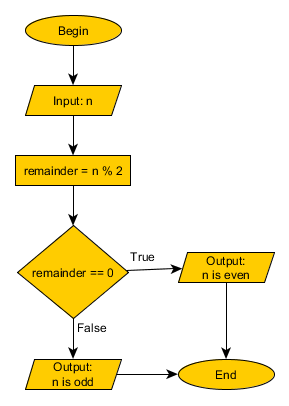
\includegraphics[width=43mm]{img/even-or-odd.png}
\end{center}
\end{column}

\begin{column}{0.4\textwidth}
\begin{python}
if n%2 == 0:
 	print('even')
else: 
 	print('odd')

\end{python}

\end{column}
\end{columns}
\end{frame}

\begin{frame}
\section{Programming languages}
\centering
\alert{Programming languages}
\end{frame}

\begin{frame}
\frametitle{History of (some) flagship languages (1/2)}

\begin{center}
\begin{tabular}{clp{79mm}}
\hline
\bf year	& \bf language	& \bf highlights	\\
\hline
1957	& Fortran	& Compiled, imperative	\\
1959	& Lisp*		& Object-oriented, popular in AI, recursive functions	\\
1964	& Basic*	& Procedural, object-oriented (``goto'')	\\
1970	& Pascal*	& Imperative, procedural, lists, trees	\\
1972	& C*		& Procedural, recursion, static type system	\\
1983	& C$^{++}$*		& Object-oriented, compiled, functional	\\
\hline
\end{tabular}
\end{center}

\bigskip
$^*$ language I ``speak'' (or ``spoke'' at some point in time)
\end{frame}

\begin{frame}
\frametitle{History of (some) flagship languages (2/2)}

\begin{center}
\begin{tabular}{clp{79mm}}
\hline
\bf year	& \bf language	& \bf highlights	\\
\hline
1989	& \red{Python}*	& Interpreted, object-oriented, code readability	\\
1995	& Java*			& Compiled, object-oriented	\\
1995	& Javascript	&Just-in-time-compiled, object-oriented, WWW	\\
1995	& PHP*			& Scripting, Web-oriented	\\
2001	& V. Basic.NET	& Object-oriented, .NET framework	\\
2009	& Go			& Compiled, C-like (safer)	\\
\hline
\end{tabular}
\end{center}

\bigskip
$^*$ language I ``speak'' (or ``spoke'' at some point in time)
\end{frame}

\begin{frame}
\frametitle{Python}
\framesubtitle{(Among other things), python is\ldots}

\alert{General-purpose}

Applicable across application domains
\bigskip 	\pause

\alert{High-level}

Strong abstraction from the computer (hardware)
\bigskip 	\pause

\alert{Interpreted}

No previous compilation into machine-level instructions necessary
\bigskip 	\pause

\alert{(Not-necessarily) object-oriented paradigm}

An object contains data (attributes) and procedures (methods)
\end{frame}

\begin{frame}
\frametitle{Python}
\framesubtitle{Some notable features}



\begin{itemize}
\item Elegant syntax (indentation-based) $\rightarrow$ easy to read	\pause 
\item Simple and ideal for prototyping	\pause 
\item It has a large standard library for diverse tasks (e.g., web servers, 
text search and processing, file reading/modifying)	\pause 
\item Interactive mode $\rightarrow$ continuous snippet testing	\pause 
\item Extendable with modules in compiled languages (e.g., C++)	\pause 
\item Multi-platform (e.g., Mac OS X, GNU Linux, Unix, MS Windows)	\pause 
\item Free: zero-cost to download/use; open-source license	\pause 
\item Large and friendly community
\end{itemize}
\bigskip 

\onslide 
\light{\url{https://wiki.python.org/moin/BeginnersGuide/Overview}}
\end{frame}

\begin{frame}
\frametitle{Python}
\framesubtitle{Some programming-language features}

\begin{itemize}
\item A variety of basic data types are available:%
\footnote{Later today}
\begin{itemize}
 \item numbers (floating point, complex, integers)
 \item strings (both ASCII and Unicode)
 \item Lists
 \item Dictionaries
\end{itemize}			\pause 
 
\item It supports object-oriented programming

\item Code can be grouped into modules and packages
\end{itemize}
\end{frame}

\begin{frame}
\frametitle{Python}
\framesubtitle{Some ways to code/launch a python program}

UNIX / GNU Linux / Windows terminal

\begin{center}
 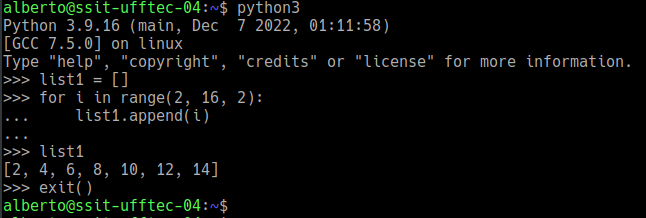
\includegraphics[width=81mm]{img/python_on_konsole.png}
\end{center}
\end{frame}

\begin{frame}
\frametitle{Python}
\framesubtitle{Some ways to code/launch a python program}

Web browser: local, online, on Google's colab

\begin{center}
 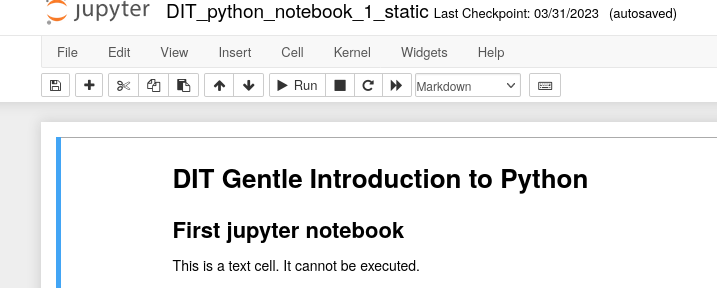
\includegraphics[width=101mm]{img/python_on_jupyter.png}
\end{center}
\end{frame}

\begin{frame}
\frametitle{Python}
\framesubtitle{Some ways to code/launch a python program}

From your web browser on DIT’s magamago (remotely online)%
\footnote{Open to advanced students only}

\begin{center}
 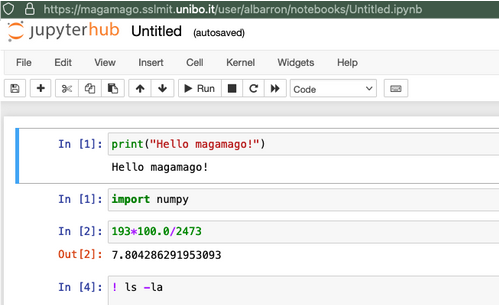
\includegraphics[width=91mm]{img/python_on_magamago.png}
\end{center}
\end{frame}

\begin{frame}
% \frametitle{Multilingual models}

\begin{center}
 \alert{Enough! Let us look at some code!}
\end{center}
\end{frame}

\begin{frame}
\section{Baby steps into coding}
\centering
\alert{Baby steps into coding}
\end{frame}

\begin{frame}
\frametitle{Google’s colab}

\begin{quote}
a free Jupyter notebook environment that runs in the cloud and stores its 
notebooks on Google Drive
\end{quote}

\begin{flushright}
\light{\url{https://colab.research.google.com}}
\end{flushright}				\pause 

\begin{center}
 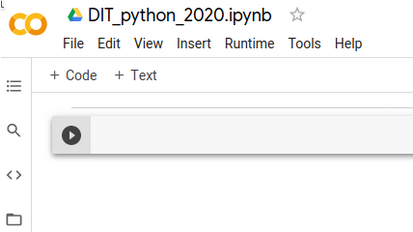
\includegraphics[width=71mm]{img/jupyter_dit.png}
\end{center}

Our first jupyter notebook
\end{frame}

\begin{frame}
\frametitle{Google’s colab: baby steps}

\begin{enumerate}
\item Visit \url{https://colab.research.google.com}
\item Click on Github
\item Type \url{https://github.com/TinfFoil/learning_dit_python}
\item Press search
\item Select 
\alert{DIT\_python\_notebook\_1\_static.ipynb}
\end{enumerate}

\begin{center}
 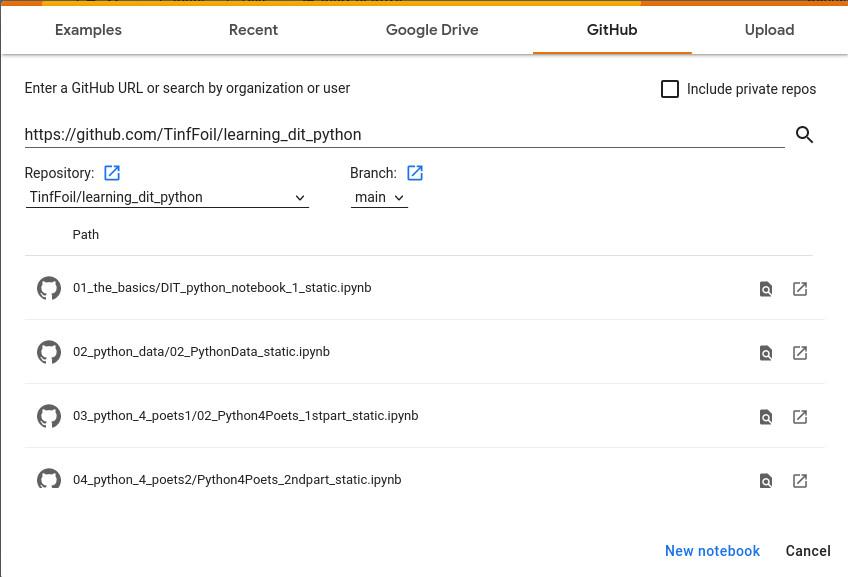
\includegraphics[width=71mm]{img/colab_git_import.png}
\end{center}
\end{frame}

\begin{frame}
\frametitle{Baby Steps}
\framesubtitle{What we know so far}

\alert{input/output}

\begin{itemize}
\item print() displays stuff to the screen
\item input() captures information from the user
\end{itemize}										\pause 

\alert{variables}
\medskip

\centering
\begin{tabular}{ll}\hline
x = 5		& x is a variable	\\
			& we assign values to a variable with = 	\\\hline	\pause 

x = 5		& is an integer	\\
x = 5.5		& is a float	\\
x = ‘ciao’	& is a string	\\
x = “ciao”	& is also a string	\\
x = ‘5’		& is \red{what?}	\\				\hline	\pause 
 
x  = x * 3	& we can apply operators to variables	\\
			& we can assign the output to a variable	\\	\hline

\end{tabular}
\end{frame}

\begin{frame}[fragile]
\frametitle{Baby Steps}
\framesubtitle{What we know so far}

\alert{flow control -- conditionals}

\begin{columns}
\begin{column}{0.4\textwidth}
\begin{python}
if (condition):
	execute something
elif (condition): 
	execute something
else: 
	execute something
\end{python}

Only \red{one} of these three snippets is executed

\end{column}				\pause 

\begin{column}{0.4\textwidth}

\begin{python}
if (condition):
 	execute something
if (condition): 
 	execute something
else: 
 	execute something
\end{python}
\alert{How is this different?}
\bigskip\medskip
\end{column}
\end{columns}			\pause 
\bigskip

\alert{flow control -- loops}

The code snippet will be executed during a number of iterations

\red{Danger}: a loop could run forever if there is an error 

\begin{columns}
\begin{column}{0.4\textwidth}
\begin{python}
for (iterator):
	execute something
\end{python}
\end{column}

\begin{column}{0.4\textwidth}
\begin{python}
while (condition):
	execute something
\end{python}
\end{column}
\end{columns}


\end{frame}
% 
\begin{frame}[fragile]
\frametitle{Baby Steps}
\framesubtitle{What we know so far}

\alert{Basic formatting}

\begin{columns}
\begin{column}{0.4\textwidth}
\begin{python}
# my code
x = 0            
while x < 50:
	for i in range(x):  
		print('x', end="")
	print()
	x += 1
\end{python}
\end{column}

\begin{column}{0.55\textwidth}
\begin{itemize}
\item Comments start with \red{\#}
\item A \red{line break} is enough to close an instruction (in Java or C, we 
need \red{;})
\item \red{Colon} opens a special code snippet
\item \red{Indentation is crucial}
\end{itemize}
\end{column}
\end{columns}
\end{frame}

\begin{frame}
\frametitle{You know a lot already!}

It is your turn to play with the notebook
\bigskip

\centering

\includegraphics[width=0.4\textwidth]{img/jupyter.png}
\end{frame}
% % 
% % \begin{frame}
% \begin{center}
% \textbf{Now go and celebrate the end of the course }
% 
% 
% 
% \ldots and worry about your project from Jan 2nd!
% \end{center}
% 
% \begin{itemize}
% 
%  \item I'm available during January for 1-to-1 discussion on your
% project \alert{upon request!}
%   \bigskip
% 
% \end{itemize}
% \end{frame}
% 
% 
% \begin{frame}[allowframebreaks]
% \frametitle{References}
% \bibliographystyle{humannat}
% \bibliography{coli}
% \end{frame}

\end{document}
